% !TEX root = task-3-11-2.tex
% Editable task bank. Append new BankTask blocks at the end of the document.
\documentclass[12pt,a4paper]{article}
\usepackage{physics-textbook}
\usepackage{graphicx,needspace}
\usetikzlibrary{decorations.pathmorphing}
\newif\ifShowSolutions
\ifdefined\TutorEdition
  \ShowSolutionstrue
\else
  \ShowSolutionsfalse % Change to \ShowSolutionstrue to display solutions.
\fi
\newcounter{banktask}
\newsavebox{\BankTaskBox}
\newcommand{\BankTaskContent}[3]{%
  \noindent\textbf{\thebanktask.}\quad #2\par
  \ifShowSolutions
    \Needspace{50mm}% Keep the solution heading with its opening text or diagram.
    #3\par
    \ifdefined\TutorEdition
      \ifcsname TutorSource#1\endcsname
        \nopagebreak\smallskip{\small\csname TutorSource#1\endcsname\par}%
      \fi
    \fi
  \fi
}
\newcommand{\BankTask}[3]{%
  \refstepcounter{banktask}\par\medskip
  \sbox{\BankTaskBox}{\begin{minipage}{\linewidth}%
    \BankTaskContent{#1}{#2}{#3}\end{minipage}}%
  \ifdim\dimexpr\ht\BankTaskBox+\dp\BankTaskBox\relax>\dimexpr\textheight-20mm\relax
    \Needspace{35mm}\BankTaskContent{#1}{#2}{#3}%
  \else
    \Needspace{\dimexpr\ht\BankTaskBox+\dp\BankTaskBox\relax}%
    \noindent\usebox{\BankTaskBox}\par
  \fi
  \medskip
}
\begin{document}
\BookSubsection{3.11.2}{Мощность тока}


% Source sdamgia-6734: https://phys-ege.sdamgia.ru/problem?id=6734
\BankTask{sdamgia-6734}{
Электрический чайник мощностью $2{,}2$ кВт рассчитан на включение в электрическую сеть напряжением $220$ В. Определите силу тока в нагревательном элементе чайника при его работе в такой сети. Ответ приведите в амперах.
}{
\smallskip\noindent\textbf{Решение}\par
Электрическую мощность можно рассчитать по формуле:$N=I ^2 R=UI,$ откуда $I= \frac{N}{U} = \frac{2{,}2 \cdot  10 ^3\,\text{Вт}}{220\,\text{В}} =10\,\text{А}.$

Ответ: $10$.
}

% Source sdamgia-7291: https://phys-ege.sdamgia.ru/problem?id=7291
\BankTask{sdamgia-7291}{
На цоколе электрической лампы накаливания написано: «$220$ В, $60\,\text{Вт}$». Две такие лампы соединяют параллельно и подключают к напряжению $127$ В. Какая мощность будет выделяться в двух этих лампах при таком способе подключения? (Ответ дать в ваттах, округлив до целых.) При решении задачи считайте, что сопротивление лампы не зависит от приложенного к ней напряжения.
}{
\smallskip\noindent\textbf{Решение}\par
Электрическая мощность $P= \frac{U ^2}{R} .$ Отсюда находим сопротивление лампочки: $R= \frac{U ^2}{P} =806{,}7\,\text{Ом}.$ При параллельном соединении сопротивление участка цепи находится по формуле: $\frac{1}{R_{\text{общ}}} = \frac{1}{R_1} + \frac{1}{R_2} .$ В нашем случае сопротивления лампочек равны и суммарное сопротивление $R_{\text{общ}}=403{,}3\,\text{Ом}.$

Воспользуемся формулой для мощности: $P= \frac{127 ^2}{403{,}3} =40\,\text{Вт}.$

Ответ: $40$.
}

% Source sdamgia-8527: https://phys-ege.sdamgia.ru/problem?id=8527
\BankTask{sdamgia-8527}{
Резистор с сопротивлением $R$ подключают к источнику тока с ЭДС $\mathcal E_1$ и внутренним сопротивлением $r_1.$ Если подключить этот резистор к источнику тока с ЭДС $\mathcal E_2 = 2\mathcal E_1$ и внутренним сопротивлением $r_2= r_1,$ то во сколько раз увеличится мощность, выделяющаяся в этом резисторе?
}{
\smallskip\noindent\textbf{Решение}\par
Согласно закону Ома для полной цепи сила тока, текущего через резистор, равна $I= \frac{\mathcal E}{R + r} .$ Следовательно, мощность, выделяющаяся в резисторе: $P=I ^2 R= \frac{\mathcal E ^2 R}{( R + r ) ^2} .$ Таким образом, поскольку $r_2= r_1,$ а $\mathcal E_2 = 2\mathcal E_1$ заключаем, что выделяемая на резисторе мощность увеличится в $4$ раза. Обратите внимание, что зависимость данной величины от внутреннего сопротивления источника менее тривиальна.

Ответ: $4$.
}

% Source sdamgia-9741: https://phys-ege.sdamgia.ru/problem?id=9741
\BankTask{sdamgia-9741}{
Два последовательно соединенных резистора сопротивлениями $4$ Ом и $8$ Ом подключены к аккумулятору, напряжение на клеммах которого равно $24$ В. Какая тепловая мощность выделяется в резисторе большего номинала?
}{
\smallskip\noindent\textbf{Решение}\par
Резисторы подключены последовательно, а, значит, полное сопротивление цепи представляет собой сумму сопротивлений резисторов. По закону Ома в цепи течет ток, по величине равный:

$I = \frac{U}{R} = \frac{24}{4 + 8} =2$ А.

На резисторе с большим сопротивлением выделится тепловая мощность:

$P=I ^2 R=2 ^2 \cdot  8 = 32$ Вт.

Ответ: $32$.
}

% Source sdamgia-10947: https://phys-ege.sdamgia.ru/problem?id=10947
\BankTask{sdamgia-10947}{
Первую лампочку мощностью $60\,\text{Вт}$ подключили к источнику постоянного напряжения $240$ В, на которое она и рассчитана. Вторую лампочку мощностью $100\,\text{Вт}$ подключили к источнику постоянного напряжения $200$ вольт, на которое она рассчитана. Во сколько раз отличается сила тока, текущего через первую лампочку, от силы тока, текущего через вторую лампочку, в рабочем режиме?
}{
\smallskip\noindent\textbf{Решение}\par
По закону Джоуля-Ленца мощность тока, которая выделяется в проводнике равна:

\[P=IU.\]

Поэтому силы токов отличаются в:

\[\frac{I_1}{I_2} = \frac{U_2P_1}{U_1P_2} = \frac{200 \cdot  60}{240 \cdot  100} =0{,}5\,\text{раза}.\]

Ответ: $0{,}5$.
}

% Source sdamgia-24103: https://phys-ege.sdamgia.ru/problem?id=24103
\BankTask{sdamgia-24103}{
Лампа накаливания подключена к источнику напряжения. После увеличения напряжения на лампе в $3$ раза выделяющаяся в ней мощность возросла в $6$ раз. Во сколько раз при этом увеличилось сопротивление спирали лампы? Ответ округлите до десятых долей.
}{
\smallskip\noindent\textbf{Решение}\par
По условию $U_{2}$ = $3$$U_{1}$, а $P_{2}$ = $6$$P_{1}$. Из формулы мощности $P= \frac{U ^2}{R} \Rightarrow R= \frac{U ^2}{P} .$ Отсюда находим отношение сопротивлений $\frac{R_2}{R_1} = \frac{9}{6} =1{,}5.$

Ответ: $1{,}5$.
}

% Source sdamgia-35994: https://phys-ege.sdamgia.ru/problem?id=35994
\BankTask{sdamgia-35994}{
Через первый резистор сопротивлением $R$ течет постоянный электрический ток силой I. Через второй резистор сопротивлением $8$R течет постоянный электрический ток силой $\frac{I}{2} .$ Чему равно отношение мощностей $\frac{P_2}{P_1} ,$ выделяющихся во втором и в первом резисторах?
}{
\smallskip\noindent\textbf{Решение}\par
Мощность тока определяется по формуле $P = I ^2 R.$ Тогда отношение мощностей равно:

\[\frac{P_2}{P_1} = \frac{I ^2 \cdot  8R}{4I ^2 \cdot  R} = 2.\]

Ответ: $2$.
}

% Source sdamgia-31890: https://phys-ege.sdamgia.ru/problem?id=31890
\BankTask{sdamgia-31890}{
К концам длинного цилиндрического однородного провода приложено напряжение U. Провод укоротили вдвое, а приложенное напряжение уменьшили в $2$ раза. Как в результате изменятся при этом сила тока в проводе и выделяющаяся в нем мощность?

Для каждой величины определите соответствующий характер изменения.

$1$. Увеличится.

$2$. Уменьшится.

$3$. Не изменится.

 

\begin{center}\small\renewcommand{\arraystretch}{1.25}\begin{tabular}{|p{0.450\linewidth}|p{0.450\linewidth}|}\hline
Сила тока & Мощность, выделяющаяся в проводе\\\hline
 & \\\hline
\end{tabular}\end{center}
}{
\smallskip\noindent\textbf{Решение}\par
При уменьшении длины проводника в $2$ раза его сопротивление уменьшится в $2$ раза. Сила тока по закону Ома для участка цепи $I= \frac{U}{R}$ при уменьшении напряжения и сопротивления в $2$ раза не изменится ($3$).

Мощность тока $P=I ^2 R$ соответственно уменьшится в $2$ раза ($2$).

Ответ: $32$.
}

% Source sdamgia-16855: https://phys-ege.sdamgia.ru/problem?id=16855
\BankTask{sdamgia-16855}{
На плавком предохранителе указано: «$30$ А». Какова максимальная суммарная мощность электрических приборов, которые можно одновременно включить в сеть с напряжением $36$ В, чтобы предохранитель не расплавился? Ответ приведите в ваттах.
}{
\smallskip\noindent\textbf{Решение}\par
Мощность вычисляется по формуле: $P = IU.$ Таким образом, предельная мощность равна $P = 36\,\text{В} \cdot  30\,\text{А} = 1080\,\text{Вт}.$

Ответ: $1080$.
}

% Source sdamgia-1925: https://phys-ege.sdamgia.ru/problem?id=1925
\BankTask{sdamgia-1925}{
На входе в электрическую цепь квартиры стоит предохранитель, размыкающий цепь при силе тока $20$ А. Подаваемое в цепь напряжение равно $220$ В. Какое максимальное количество утюгов, мощность каждого из которых равна $400\,\text{Вт}$, можно одновременно включить в квартире?
}{
\smallskip\noindent\textbf{Решение}\par
Все утюги включаются параллельно друг к другу, поэтому на каждый из них подается одинаковое напряжение, а токи складываются. Предохранитель, стоящий в цепи, размыкается при мощности, потребляемой всеми утюгами $P=UI=220\,\text{В} \cdot  20\,\text{А}=4400\,\text{Вт}.$ Каждый утюг потребляет мощность $400\,\text{Вт}$, следовательно, при включении $( 4400\,\text{Вт} ) / ( 400\,\text{Вт} ) =11$ утюгов и более цепь разомкнется. Утюгов должно быть $10$, чтобы они работали без размыкания цепи.

Ответ: $10$.
}


% Source De83D5: https://ege.fipi.ru/bank/questions.php?search=1&proj=BA1F39653304A5B041B656915DC36B38&qid=De83D5
\BankTask{De83D5}{
На рисунке показан график зависимости силы тока в лампе накаливания от напряжения на её клеммах. Определите мощность тока в лампе при силе тока, равной $1{,}5\,\text{А}$.
\begin{center}
\begin{tikzpicture}[x=0.15cm,y=1.5cm,>=stealth]
\draw[thin] (0,0) grid[xstep=5,ystep=0.5] (35,2.5);
\draw (0,0)--(35,0) node[right] {$U,\,\text{В}$};
\draw[->] (0,0)--(0,2.9) node[left] {$I,\,\text{А}$};
\node[below left] at (0,0) {$0$};
\foreach \x in {10,20,30} \node[below] at (\x,0) {$\x$};
\foreach \y in {1,2} \node[left] at (0,\y) {$\y$};
\draw[very thick] (0,0) .. controls (3,0.35) and (6.5,0.68) .. (10,0.94) .. controls (13.5,1.18) and (17,1.38) .. (20,1.5) .. controls (25,1.7) and (30,1.9) .. (35,2);
\end{tikzpicture}
\end{center} (в $\text{Вт}$).
}{
\smallskip\noindent\textbf{Решение от GPT}\par
По графику при $I=1{,}5\,\text{А}$ напряжение $U=20\,\text{В}$. Мощность тока:
\[
P=UI=20\cdot1{,}5=30\,\text{Вт}.
\]
Ответ: $30\,\text{Вт}$.
}

% Source 0AEE10: https://ege.fipi.ru/bank/questions.php?search=1&proj=BA1F39653304A5B041B656915DC36B38&qid=0AEE10
\BankTask{0AEE10}{
На колбе лампы накаливания указано: «\(165\ \text{Вт},\ 220\ \text{В}\)». Найдите силу тока в спирали при включении лампы в сеть с таким напряжением. (в $\text{А}$).
}{
\smallskip\noindent\textbf{Решение от GPT}\par
Из \(P=UI\) получаем
\[
I=\frac{P}{U}=\frac{165}{220}=0{,}75\ \text{А}.
\]
Ответ: \(0{,}75\ \text{А}\).
}

% Source D474CD: https://ege.fipi.ru/bank/questions.php?search=1&proj=BA1F39653304A5B041B656915DC36B38&qid=D474CD
\BankTask{D474CD}{
На плавком предохранителе указано: «\(30\ \text{А}\)». Какова максимальная суммарная мощность электрических приборов, которые можно одновременно включить в сеть с напряжением \(36\ \text{В}\), чтобы предохранитель не расплавился (в $\text{Вт}$)?
}{
\smallskip\noindent\textbf{Решение от GPT}\par
Суммарный ток не должен превышать \(I_{\max}=30\ \text{А}\). Поэтому
\[
P_{\max}=UI_{\max}=36\cdot30=1080\ \text{Вт}.
\]
Ответ: \(1080\ \text{Вт}\).
}

% Source 5D79D1: https://ege.fipi.ru/bank/questions.php?search=1&proj=BA1F39653304A5B041B656915DC36B38&qid=5D79D1
\BankTask{5D79D1}{
При нагревании спирали лампы накаливания протекающим по ней электрическим током основная часть подводимой энергии теряется в виде теплового излучения. На рисунке изображены графики зависимости мощности тепловых потерь лампы от температуры спирали $P=P(T)$ и силы тока от приложенного напряжения $I=I(U)$.
\begin{enumerate}
\item С уменьшением приложенного напряжения температура спирали уменьшается пропорционально мощности.
\item При напряжении $100\,\text{В}$ сопротивление спирали лампы равно $50\,\text{Ом}$.
\item Сопротивление спирали лампы постоянно и не зависит от температуры.
\item Температура спирали лампы при приложенном напряжении $U=120\,\text{В}$ меньше $3600\,\text{К}$.
\item С увеличением силы протекающего тока температура спирали увеличивается.
\end{enumerate}
\begin{center}
\begin{tikzpicture}[book diagram,x=1cm,y=1cm]
\begin{scope}
\draw[thin,step=0.5] (0,0) grid (4,2.5);
\draw[-{book tip}] (0,0)--(4.85,0) node[below] {$T,\,\text{К}$};
\draw[-{book tip}] (0,0)--(0,2.95) node[left] {$P,\,\text{Вт}$};
\foreach \x/\t in {0/2000,1/2400,2/2800,3/3200,4/3600}{\node[below,font=\small] at (\x,0) {$\t$};}
\foreach \y/\p in {0/0,1/100,2/200}{\node[left,font=\small] at (0,\y) {$\p$};}
\draw[thin] plot[smooth] coordinates {(0,0.17) (0.5,0.25) (1,0.40) (1.5,0.58) (2,0.77) (2.5,1.02) (3,1.33) (3.5,1.71) (4,2.14)};
\end{scope}
\begin{scope}[xshift=6.3cm]
\draw[thin,step=0.4] (0,0) grid (4,2.8);
\draw[-{book tip}] (0,0)--(4.85,0) node[below] {$U,\,\text{В}$};
\draw[-{book tip}] (0,0)--(0,3.15) node[left] {$I,\,\text{А}$};
\foreach \x/\u in {0/50,2/100,4/150}{\node[below,font=\small] at (\x,0) {$\u$};}
\foreach \y/\i in {0/{1{,}2},0.8/{1{,}6},1.6/{2{,}0},2.4/{2{,}4}}{\node[left,font=\small] at (0,\y) {$\i$};}
\draw[thin] plot[smooth] coordinates {(0,0.4) (0.4,0.65) (0.8,0.89) (1.2,1.13) (1.6,1.37) (2,1.6) (2.4,1.82) (2.8,2.03) (3.2,2.22) (3.6,2.40) (4,2.56)};
\end{scope}
\end{tikzpicture}
\end{center}
}{
\smallskip\noindent\textbf{Решение от GPT}\par
Утверждение 1 неверно: график $P(T)$ нелинейный, поэтому температура не пропорциональна мощности. Утверждение 2 верно: при $U=100\,\text{В}$ ток $I=2\,\text{А}$, следовательно, $R=U/I=50\,\text{Ом}$. Утверждение 3 неверно: отношение $U/I$ меняется, например при $50\,\text{В}$ оно равно примерно $36\,\text{Ом}$. Утверждение 4 неверно: при $120\,\text{В}$ мощность $UI\approx264\,\text{Вт}$ превышает тепловые потери при $3600\,\text{К}$, поэтому температура выше $3600\,\text{К}$. Утверждение 5 верно: рост тока сопровождается ростом напряжения и мощности, а значит, температуры спирали. Ответ: 2, 5.
}

% Source 10C527: https://ege.fipi.ru/bank/questions.php?search=1&proj=BA1F39653304A5B041B656915DC36B38&qid=10C527
\BankTask{10C527}{
Электрическая цепь на рисунке состоит из источника постоянного напряжения с ЭДС $\mathcal{E}$ и внутренним сопротивлением $r$ и внешней цепи из двух одинаковых резисторов сопротивлением $R$, включённых параллельно. Установите соответствие между физическими величинами и формулами, по которым их можно рассчитать.

\begin{center}
\TaskMatchingColumns[0.53\linewidth]{Физические величины}{
А) мощность тока, выделяющаяся на одном из резисторов $R$\par
Б) мощность сторонних сил в источнике тока
}{Формулы}{
1) $\displaystyle\frac{\mathcal{E}^2R}{4\left(r+\frac{R}{2}\right)^2}$\par
2) $\displaystyle\frac{\mathcal{E}^2R}{2\left(r+\frac{R}{2}\right)^2}$\par
3) $\displaystyle\frac{\mathcal{E}^2r}{\left(r+\frac{R}{2}\right)^2}$\par
4) $\displaystyle\frac{\mathcal{E}^2}{r+\frac{R}{2}}$
}

\medskip
\begin{tabular}{|c|c|}
\hline
А & Б \\
\hline
\phantom{1} & \phantom{1} \\
\hline
\end{tabular}
\end{center}

\begin{center}
\begin{tikzpicture}[book diagram,x=0.8cm,y=0.8cm]
\draw (0,1.9)--(0,3.5)--(4.6,3.5)--(4.6,2.45);
\draw (0,1.55)--(0,0)--(4.6,0)--(4.6,1.1);
\draw (-0.55,1.9)--(0.55,1.9);
\draw (-0.3,1.55)--(0.3,1.55);
\node[left] at (-0.55,2.35) {$\mathcal{E},r$};
\draw (2.3,3.5)--(2.3,2.45);
\draw (1.975,1.1) rectangle (2.625,2.45);
\draw (2.3,1.1)--(2.3,0);
\node[right] at (2.65,1.775) {$R$};
\draw (4.275,1.1) rectangle (4.925,2.45);
\node[right] at (4.95,1.775) {$R$};
\fill (2.3,3.5) circle (1.5pt);
\fill (2.3,0) circle (1.5pt);
\end{tikzpicture}
\end{center}
}{
\smallskip\noindent\textbf{Решение от GPT}\par
Сопротивление внешней цепи равно $R/2$, поэтому ток через источник $I=\mathcal{E}/(r+R/2)$. Через каждый резистор течёт ток $I/2$, и мощность одного резистора равна $P_R=I^2R/4=\mathcal{E}^2R/[4(r+R/2)^2]$, то есть А — 1. Мощность сторонних сил $P_{\text{ст}}=\mathcal{E}I=\mathcal{E}^2/(r+R/2)$, то есть Б — 4. Ответ: $14$.
}

% Source BB603A: https://ege.fipi.ru/bank/questions.php?search=1&proj=BA1F39653304A5B041B656915DC36B38&qid=BB603A
\BankTask{BB603A}{
Электрическая цепь на рисунке состоит из источника постоянного напряжения с ЭДС $\mathcal{E}$ и внутренним сопротивлением $r$ и внешней цепи из двух одинаковых резисторов сопротивлением $R$, включённых параллельно. Установите соответствие между физическими величинами и формулами, по которым их можно рассчитать.

\begin{center}
\TaskMatchingColumns[0.53\linewidth]{Физические величины}{
А) мощность тока, выделяющаяся во внешней цепи из двух резисторов $R$\par
Б) мощность тока, выделяющаяся на внутреннем сопротивлении источника тока
}{Формулы}{
1) $\displaystyle\frac{\mathcal{E}^2R}{4\left(r+\frac{R}{2}\right)^2}$\par
2) $\displaystyle\frac{\mathcal{E}^2R}{2\left(r+\frac{R}{2}\right)^2}$\par
3) $\displaystyle\frac{\mathcal{E}^2r}{\left(r+\frac{R}{2}\right)^2}$\par
4) $\displaystyle\frac{\mathcal{E}^2}{r+\frac{R}{2}}$
}

\medskip
\begin{tabular}{|c|c|}
\hline
А & Б \\
\hline
\phantom{1} & \phantom{1} \\
\hline
\end{tabular}
\end{center}

\begin{center}
\begin{tikzpicture}[book diagram,x=0.8cm,y=0.8cm]
\draw (0,1.9)--(0,3.5)--(4.6,3.5)--(4.6,2.45);
\draw (0,1.55)--(0,0)--(4.6,0)--(4.6,1.1);
\draw (-0.55,1.9)--(0.55,1.9);
\draw (-0.3,1.55)--(0.3,1.55);
\node[left] at (-0.55,2.35) {$\mathcal{E},r$};
\draw (2.3,3.5)--(2.3,2.45);
\draw (1.975,1.1) rectangle (2.625,2.45);
\draw (2.3,1.1)--(2.3,0);
\node[right] at (2.65,1.775) {$R$};
\draw (4.275,1.1) rectangle (4.925,2.45);
\node[right] at (4.95,1.775) {$R$};
\fill (2.3,3.5) circle (1.5pt);
\fill (2.3,0) circle (1.5pt);
\end{tikzpicture}
\end{center}
}{
\smallskip\noindent\textbf{Решение от GPT}\par
Эквивалентное сопротивление двух параллельных резисторов равно $R/2$, поэтому $I=\mathcal{E}/(r+R/2)$. Во внешней цепи выделяется мощность $P_{\text{внеш}}=I^2R/2=\mathcal{E}^2R/[2(r+R/2)^2]$, что соответствует формуле 2. На внутреннем сопротивлении выделяется мощность $P_r=I^2r=\mathcal{E}^2r/(r+R/2)^2$, что соответствует формуле 3. Ответ: $23$.
}

% Source 433A84: https://ege.fipi.ru/bank/questions.php?search=1&proj=BA1F39653304A5B041B656915DC36B38&qid=433A84
\BankTask{433A84}{
Электрическая цепь, схема которой изображена на рисунке, подключена к аккумулятору. Напряжение между полюсами аккумулятора равно \(U_0\), а показания идеальных амперметра и вольтметра равны соответственно \(I\) и \(U\).

Установите соответствие между физическими величинами и формулами, по которым их можно рассчитать. Внутренним сопротивлением аккумулятора пренебречь.

\TaskMatchingColumns[0.59\linewidth]{Физические величины}{
А) мощность, потребляемая лампочкой\par
Б) сопротивление лампочки
}{Формулы}{
1) \(\dfrac{U}{I}\)\par
2) \(\dfrac{U_0-U}{I}\)\par
3) \((U_0-U)I\)\par
4) \(UI\)
}

\begin{center}
\begin{tabular}{|c|c|}
\hline
А & Б \\
\hline
\phantom{3} & \phantom{2} \\
\hline
\end{tabular}
\end{center}

\begin{center}
\begin{tikzpicture}[book diagram, x=1cm, y=1cm, line width=0.8pt]
\draw (1.15,1.5) -- (0,1.5) -- (0,1.05);
\draw (0,0.45) -- (0,0) -- (0.5,0);
\draw (0,0.75) circle (0.3);
\node at (0,0.75) {\(\mathrm{A}\)};
\draw (0.8,0) circle (0.3);
\draw (0.59,-0.21) -- (1.01,0.21);
\draw (0.59,0.21) -- (1.01,-0.21);
\draw (1.1,0) -- (1.5,0) -- (2,0);
\draw (2,-0.15) rectangle (2.6,0.15);
\draw (2.6,0) -- (3.05,0) -- (3.05,1.5) -- (1.8,1.5);
\draw (1.5,0) -- (1.5,0.9) -- (1.95,0.9);
\draw (2.25,0.9) circle (0.3);
\node at (2.25,0.9) {\(\mathrm{V}\)};
\draw (2.55,0.9) -- (3.05,0.9);
\fill (1.5,0) circle (0.045);
\fill (3.05,0.9) circle (0.045);
\draw[fill=white] (1.15,1.5) circle (0.06);
\draw[fill=white] (1.8,1.5) circle (0.06);
\node at (1.475,1.88) {\(U_0\)};
\end{tikzpicture}
\end{center}
}{
\smallskip\noindent\textbf{Решение от GPT}\par
Идеальный вольтметр измеряет напряжение на резисторе и не пропускает ток, поэтому через лампочку течёт ток \(I\), а напряжение на ней равно \(U_0-U\). Мощность лампочки \(P=(U_0-U)I\) соответствует формуле 3, её сопротивление \(R=\dfrac{U_0-U}{I}\) — формуле 2. Формулы 1 и 4 определяют соответственно сопротивление и мощность резистора. Ответ: \(32\).
}

% Source BD62B3: https://ege.fipi.ru/bank/questions.php?search=1&proj=BA1F39653304A5B041B656915DC36B38&qid=BD62B3
\BankTask{BD62B3}{
Установите соответствие между формулами для расчёта физических величин в цепях постоянного тока и названиями этих величин. В формулах использованы обозначения: \(R\) — сопротивление резистора; \(P\) — мощность тока в резисторе; \(U\) — напряжение на резисторе.

\TaskMatchingColumns[.35\linewidth]{Формулы}{
А) \(\dfrac{U}{R}\)\par
Б) \(\dfrac{U^2}{P}\)
}{Физические величины}{
1) мощность тока в резисторе\par
2) сопротивление резистора\par
3) сила тока\par
4) количество теплоты, выделяющееся в резисторе
}

\begin{center}
\begin{tabular}{|c|c|}
\hline
А & Б \\
\hline
\phantom{3} & \phantom{2} \\
\hline
\end{tabular}
\end{center}
}{
\smallskip\noindent\textbf{Решение от GPT}\par
По закону Ома \(I=\dfrac{U}{R}\), поэтому А соответствует силе тока (3). Из формулы мощности \(P=\dfrac{U^2}{R}\) получаем \(R=\dfrac{U^2}{P}\), поэтому Б соответствует сопротивлению (2). Мощность (1) равна \(UI\), а количество теплоты (4) равно \(Pt\); ни одна из данных формул их не определяет. Ответ: \(32\).
}

% Source 9040: https://phys-ege.sdamgia.ru/problem?id=9040
\BankTask{9040}{
На рисунке изображены две электрические цепи. Первая содержит последовательно соединенные источник тока ($1$), реостат, катушку индуктивности и амперметр, а вторая  — проволочный моток, к концам которого присоединен гальванометр, изображенный на рисунке справа. Катушка и моток надеты на железный сердечник ($2$).

\begin{center}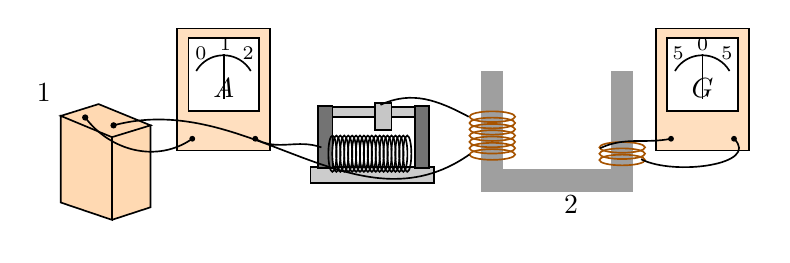
\begin{tikzpicture}[>=stealth,line width=.6pt]

\draw[fill=orange!30] (0,0)--(0,1.1)--(.65,.83)--(.65,-.22)--cycle (.65,.83)--(1.14,.98)--(1.14,-.06)--(.65,-.22) (0,1.1)--(.48,1.25)--(1.14,.98)--(.65,.83)--cycle;
\node[above left] at (0,1.16) {$1$};\fill(.31,1.08)circle(.04) (.67,.98)circle(.04);
\draw[fill=orange!25] (1.48,.66) rectangle (2.66,2.21) (7.56,.66) rectangle (8.74,2.21);
\foreach \x/\s in {2.07/A,8.15/G}{\draw[fill=white](\x-.45,1.16)rectangle(\x+.45,2.09);\draw(\x-.35,1.67) arc(150:30:.4);\draw(\x,1.32)--(\x,1.88);\node at(\x,1.45){$\s$};\fill(\x-.4,.81)circle(.037) (\x+.4,.81)circle(.037);}
\node at(1.78,1.9){\scriptsize $0$};\node at(2.09,2.01){\scriptsize $1$};\node at(2.38,1.9){\scriptsize $2$};
\node at(8.15,2.01){\scriptsize $0$};\node at(7.84,1.9){\scriptsize $5$};\node at(8.46,1.9){\scriptsize $5$};
\draw[fill=gray!40](3.17,.25)rectangle(4.74,.45) (3.29,1.09)rectangle(4.62,1.21);
\draw[fill=black!55](3.27,.44) rectangle(3.45,1.23) (4.5,.44)rectangle(4.68,1.23);
\foreach \x in {3.45,3.5,...,4.45}{\draw (\x,.62) ellipse(.052 and .23);}
\draw[fill=gray!45](3.99,.92) rectangle(4.2,1.26);
\draw[draw=gray!75,line width=8pt] (5.48,1.67)--(5.48,.28)--(7.13,.28)--(7.13,1.67);
\foreach \x/\y in {5.48/.61,5.48/.69,5.48/.77,5.48/.85,5.48/.93,5.48/1.01,5.48/1.09,7.13/.54,7.13/.62,7.13/.70}{\draw[orange!65!black] (\x,\y)ellipse(.29 and .068);}
\node[below] at(6.48,.22){$2$};
\draw(.31,1.08)to[out=-53,in=215](1.67,.81) (2.47,.81)to[out=-30,in=160](3.31,.7)
 (4.06,1.24)to[out=25,in=152](5.18,1.09) (5.19,.61)to[out=-145,in=15](.67,.98)
 (6.85,.69)to[out=25,in=191](7.75,.81) (7.37,.55)to[out=-27,in=-44](8.55,.81);

\end{tikzpicture}\end{center}

Как будут изменяться показания приборов при плавном уменьшении сопротивления реостата? Ответ поясните, указав, какие физические закономерности Вы использовали для объяснения.
}{
\smallskip\noindent\textbf{Решение}\par
$1$.  При плавном уменьшении сопротивления реостата ток в цепи будет плавно увеличиваться согласно закону Ома $I= \frac{U}{R} ,$ а значит, показания амперметра будут возрастать.
$2$.  Увеличение силы тока в цепи приведет к увеличению потока $\,\text{Ф}=LI$ вектора магнитной индукции через железный сердечник и, как следствие, приведет к возникновению небольшой ЭДС индукции $\mathcal E_{\,\text{инд}}$ в цепи этой катушки, $\mathcal E_{\,\text{инд}}\ll\mathcal E ,$ которой можно пренебречь.
$3$.  Увеличение потока вектора магнитной индукции через поперечное сечение сердечника вызовет изменение потока вектора индукции магнитного поля в проволочном мотке, соединенном с гальванометром. В соответствии с законом индукции Фарадея $\mathcal E_2= - \frac{\Delta \Phi}{\Delta t} ,$ что вызывает ток через гальванометр, вследствие чего стрелка гальванометра отклонится от начального положения.
}

% Source 25381: https://phys-ege.sdamgia.ru/problem?id=25381
\BankTask{25381}{
\begin{center}\begin{tikzpicture}[>=stealth,line width=.6pt]

\draw(0,1)--(0,1.91) (0,2.29)--(0,2.75)--(4.51,2.75)--(4.51,2.3) (4.51,1.92)--(4.51,1.0)
 (4.51,.58)--(4.51,-.14)--(0,-.14)--(0,.58)
 (1.65,2.75)--(1.65,2.29) (1.65,1.49)--(1.65,1.25) (1.65,1.11)--(1.65,.53)
 (2.91,2.75)--(2.91,1.25) (2.91,1.11)--(2.91,.53);
\fill(1.65,.53)circle(.042) (2.91,.53)circle(.042) (2.28,.24)circle(.042);
\draw (2.28,-.14)--(2.28,.24);
\node[left]at(1.65,.45){$1$};\node[right]at(2.91,.45){$2$};
\draw(2.28,.24)--(1.65,.53);\begin{scope}[shift={(0,2.1)},rotate=-90]\draw(-.2,-.16)--(-.2,.16)--(.18,0)--cycle (.18,-.18)--(.18,.18);\end{scope}\node[left] at (0,2.3000000000000003) {$\text{Д1}$};\begin{scope}[shift={(4.51,2.11)},rotate=90]\draw(-.2,-.16)--(-.2,.16)--(.18,0)--cycle (.18,-.18)--(.18,.18);\end{scope}\node[right] at (4.51,2.31) {$\text{Д2}$};\begin{scope}[shift={(0,0.79)}]\draw(0,0)circle(.21) (-.14,-.14)--(.14,.14) (-.14,.14)--(.14,-.14);\node[left]at(-.23,0){Л1};\end{scope}\begin{scope}[shift={(4.51,0.79)}]\draw(0,0)circle(.21) (-.14,-.14)--(.14,.14) (-.14,.14)--(.14,-.14);\node[left]at(-.23,0){};\end{scope}\node[right]at(4.72,.79){Л2};\begin{scope}[shift={(1.65,1.89)},rotate=90]\draw[fill=orange!35] (-.4,-.13) rectangle (.4,.13);\end{scope}\node[left] at (1.65,1.89) {$R$};\begin{scope}[shift={(1.65,1.18)},rotate=-90]\draw(-.07,-.21)--(-.07,.21) (.07,-.11)--(.07,.11);\end{scope}\node[above right] at (1.77,1.18) {$$};\begin{scope}[shift={(2.91,1.18)},rotate=90]\draw(-.07,-.21)--(-.07,.21) (.07,-.11)--(.07,.11);\end{scope}\node[above right] at (3.0300000000000002,1.18) {$$};\node[left]at(1.46,1.18){$\mathcal E,r$};\node[right]at(3.09,1.18){$\mathcal E,r$};
\end{tikzpicture}\end{center}
На рисунке изображена схема электрической цепи, состоящей из двух одинаковых источников тока с ЭДС $\mathcal{E}$ и внутренним сопротивлением r, резистора сопротивлением R, двух одинаковых ламп Л1 и Л2, двух идеальных диодов Д1 и Д2 и ключа К. Опираясь на законы электродинамики, объясните, какие изменения произойдут в работе этой цепи, если перевести ключ К из положения $1$ в положение $2$. Сравните накал ламп в этих двух случаях.
}{
\smallskip\noindent\textbf{Решение}\par
При замыкании первого ключа ток не идет через правый источник тока. В этом случае цепь будет иметь вид, показанный на рис. $1$. Направление тока от плюса к минусу. При этом через диод Д1 ток идет в прямом направлении, а через диод Д2  — в обратном. Известно, что идеальный диод обладает малым сопротивлением при прохождении тока в прямом направлении и бесконечным сопротивлением при прохождении тока в обратном направлении. Тогда эквивалентная схема будет иметь вид, показанный на рис. $2$. 
При переводе ключа во второе положение, ток не будет идти через левый источник. Цепь будет иметь вид, показанный на рис. $3$. В этом случае ток через диод Д2 будет идти в прямом направлении, а через диод Д1  — в обратном. Тогда эквивалентная схема будет иметь вид, показанный на рис. $4$. 


\begin{center}\begin{tikzpicture}[>=stealth,line width=.6pt]

\draw(0,1)--(0,1.91) (0,2.29)--(0,2.75)--(4.51,2.75)--(4.51,2.3) (4.51,1.92)--(4.51,1.0)
 (4.51,.58)--(4.51,-.14)--(0,-.14)--(0,.58)
 (1.65,2.75)--(1.65,2.29) (1.65,1.49)--(1.65,1.25) (1.65,1.11)--(1.65,.53)
 (2.91,2.75)--(2.91,1.25) (2.91,1.11)--(2.91,.53);
\fill(1.65,.53)circle(.042) (2.91,.53)circle(.042) (2.28,.24)circle(.042);
\draw (2.28,-.14)--(2.28,.24);
\node[left]at(1.65,.45){$1$};\node[right]at(2.91,.45){$2$};
\draw(2.28,.24)--(1.65,.53);\draw[->](1.57,1.55)--(1.57,2.42);\draw[->](.85,2.57)--(.1,2.57);\draw[->](.18,1.7)--(.18,1.1);\draw[->](.66,.04)--(1.4,.04);\draw[->](3.3,2.57)--(4.37,2.57);\begin{scope}[shift={(0,2.1)},rotate=-90]\draw(-.2,-.16)--(-.2,.16)--(.18,0)--cycle (.18,-.18)--(.18,.18);\end{scope}\node[left] at (0,2.3000000000000003) {$\text{Д1}$};\begin{scope}[shift={(4.51,2.11)},rotate=90]\draw(-.2,-.16)--(-.2,.16)--(.18,0)--cycle (.18,-.18)--(.18,.18);\end{scope}\node[right] at (4.51,2.31) {$\text{Д2}$};\begin{scope}[shift={(0,0.79)}]\draw(0,0)circle(.21) (-.14,-.14)--(.14,.14) (-.14,.14)--(.14,-.14);\node[left]at(-.23,0){Л1};\end{scope}\begin{scope}[shift={(4.51,0.79)}]\draw(0,0)circle(.21) (-.14,-.14)--(.14,.14) (-.14,.14)--(.14,-.14);\node[left]at(-.23,0){};\end{scope}\node[right]at(4.72,.79){Л2};\begin{scope}[shift={(1.65,1.89)},rotate=90]\draw[fill=orange!35] (-.4,-.13) rectangle (.4,.13);\end{scope}\node[left] at (1.65,1.89) {$R$};\begin{scope}[shift={(1.65,1.18)},rotate=-90]\draw(-.07,-.21)--(-.07,.21) (.07,-.11)--(.07,.11);\end{scope}\node[above right] at (1.77,1.18) {$$};\begin{scope}[shift={(2.91,1.18)},rotate=90]\draw(-.07,-.21)--(-.07,.21) (.07,-.11)--(.07,.11);\end{scope}\node[above right] at (3.0300000000000002,1.18) {$$};\node[left]at(1.46,1.18){$\mathcal E,r$};\node[right]at(3.09,1.18){$\mathcal E,r$};
\end{tikzpicture}\end{center}

Рис. $1$ 


\begin{center}\begin{tikzpicture}[>=stealth,line width=.6pt]
\draw(0,1.02)--(0,2.4)--(2.61,2.4)--(2.61,1.86) (2.61,1.06)--(2.61,.74) (2.61,.6)--(2.61,-.18)--(0,-.18)--(0,.6);\begin{scope}[shift={(0,0.81)}]\draw(0,0)circle(.21) (-.14,-.14)--(.14,.14) (-.14,.14)--(.14,-.14);\node[left]at(-.23,0){Л1};\end{scope}\begin{scope}[shift={(2.61,1.46)},rotate=90]\draw[fill=orange!35] (-.4,-.13) rectangle (.4,.13);\end{scope}\node[left] at (2.61,1.46) {$R$};\begin{scope}[shift={(2.61,0.67)},rotate=-90]\draw(-.07,-.21)--(-.07,.21) (.07,-.11)--(.07,.11);\end{scope}\node[above right] at (2.73,0.67) {$\mathcal E,r$};
\end{tikzpicture}\end{center}

Рис. $2$ 


\begin{center}\begin{tikzpicture}[>=stealth,line width=.6pt]

\draw(0,1)--(0,1.91) (0,2.29)--(0,2.75)--(4.51,2.75)--(4.51,2.3) (4.51,1.92)--(4.51,1.0)
 (4.51,.58)--(4.51,-.14)--(0,-.14)--(0,.58)
 (1.65,2.75)--(1.65,2.29) (1.65,1.49)--(1.65,1.25) (1.65,1.11)--(1.65,.53)
 (2.91,2.75)--(2.91,1.25) (2.91,1.11)--(2.91,.53);
\fill(1.65,.53)circle(.042) (2.91,.53)circle(.042) (2.28,.24)circle(.042);
\draw (2.28,-.14)--(2.28,.24);
\node[left]at(1.65,.45){$1$};\node[right]at(2.91,.45){$2$};
\draw(2.28,.24)--(2.91,.53);\draw[->](3.8,2.57)--(3.2,2.57);\draw[->](3.08,1.0)--(3.08,.27);\draw[->](4.36,1.24)--(4.36,1.86);\draw[->](2.15,.04)--(1.5,.04);\draw[->](.16,1.22)--(.16,1.79);\begin{scope}[shift={(0,2.1)},rotate=-90]\draw(-.2,-.16)--(-.2,.16)--(.18,0)--cycle (.18,-.18)--(.18,.18);\end{scope}\node[left] at (0,2.3000000000000003) {$\text{Д1}$};\begin{scope}[shift={(4.51,2.11)},rotate=90]\draw(-.2,-.16)--(-.2,.16)--(.18,0)--cycle (.18,-.18)--(.18,.18);\end{scope}\node[right] at (4.51,2.31) {$\text{Д2}$};\begin{scope}[shift={(0,0.79)}]\draw(0,0)circle(.21) (-.14,-.14)--(.14,.14) (-.14,.14)--(.14,-.14);\node[left]at(-.23,0){Л1};\end{scope}\begin{scope}[shift={(4.51,0.79)}]\draw(0,0)circle(.21) (-.14,-.14)--(.14,.14) (-.14,.14)--(.14,-.14);\node[left]at(-.23,0){};\end{scope}\node[right]at(4.72,.79){Л2};\begin{scope}[shift={(1.65,1.89)},rotate=90]\draw[fill=orange!35] (-.4,-.13) rectangle (.4,.13);\end{scope}\node[left] at (1.65,1.89) {$R$};\begin{scope}[shift={(1.65,1.18)},rotate=-90]\draw(-.07,-.21)--(-.07,.21) (.07,-.11)--(.07,.11);\end{scope}\node[above right] at (1.77,1.18) {$$};\begin{scope}[shift={(2.91,1.18)},rotate=90]\draw(-.07,-.21)--(-.07,.21) (.07,-.11)--(.07,.11);\end{scope}\node[above right] at (3.0300000000000002,1.18) {$$};\node[left]at(1.46,1.18){$\mathcal E,r$};\node[right]at(3.09,1.18){$\mathcal E,r$};
\end{tikzpicture}\end{center}

Рис. $3$ 


\begin{center}\begin{tikzpicture}[>=stealth,line width=.6pt]
\draw(0,1.04)--(0,2.37)--(2.61,2.37)--(2.61,1.18) (2.61,.76)--(2.61,-.18)--(0,-.18)--(0,.9);\begin{scope}[shift={(2.61,0.97)}]\draw(0,0)circle(.21) (-.14,-.14)--(.14,.14) (-.14,.14)--(.14,-.14);\node[left]at(-.23,0){Л2};\end{scope}\begin{scope}[shift={(0,0.97)},rotate=90]\draw(-.07,-.21)--(-.07,.21) (.07,-.11)--(.07,.11);\end{scope}\node[above right] at (0.12,0.97) {$$};\node[left]at(-.24,.97){$\mathcal E,r$};
\end{tikzpicture}\end{center}

Рис. $4$ 

В первом случае в цепи лампа Л1 и резистор соединены последовательно. Их общее сопротивление равно $R + R_{\,\text{л}}.$ По закону Ома для полной цепи, сила тока $I_1= \frac{\mathcal{E}}{R + R_{\,\text{л}} + r} .$
Во втором случае в цепи будет только лампа Л2. По закону Ома для полной цепи сила тока $I_2= \frac{\mathcal{E}}{R_{\,\text{л}} + r} .$ Очевидно, что сопротивление уменьшилось, а сила тока увеличилась. Мощность тока в первом случае:

\[P_1=I_1 ^2 R_{\,\text{л}}= \frac{\mathcal E^2 R_{\text{л}}}{(R+R_{\text{л}}+r)^2} ,\]

во втором случае:

\[P_2=I_2 ^2 R_{\,\text{л}}= \frac{\mathcal E^2 R_{\text{л}}}{(R_{\text{л}}+r)^2} .\]

Из приведенных формул видно, что мощность тока увеличилась, следовательно, при переводе ключа из положения $1$ в положение $2$ накал одной из ламп увеличится, а другая лампа гореть не будет.

Ответ: накал горящей лампы увеличится.
}

% Source 11810: https://phys-ege.sdamgia.ru/problem?id=11810
\BankTask{11810}{
\begin{center}\begin{tikzpicture}[>=stealth,line width=.6pt]

\draw[task grid,step=.46] (0,0) grid (3.22,2.76);
\draw[task axis] (0,0)--(3.39,0) node[right] {$U,\,\text{В}$};
\draw[task axis] (0,0)--(0,2.93) node[above left] {$P,\,\text{Вт}$};
\foreach \x in {0,...,6}{\node[below] at (.46*\x,0) {$\x$};}
\foreach \y in {1,...,4}{\node[left] at (0,.46*\y) {$\y$};}
\draw[task curve,orange!85!black,domain=0:2.76,samples=80] plot(\x,{(2.3/1.9044)*\x*(2.76-\x)});

\end{tikzpicture}\end{center}
Электрическая цепь состоит из батареи с ЭДС \ensuremath{\mathcal E} и внутренним сопротивлением r и подключенного к ней резистора нагрузки с сопротивлением R. При изменении сопротивления нагрузки изменяется напряжение на ней и мощность в нагрузке. На рисунке представлен график зависимости мощности, выделяющейся на нагрузке, от напряжения на ней. Используя известные Вам физические законы, объясните, почему данный график зависимости мощности от напряжения представляет собой параболу.
}{
\smallskip\noindent\textbf{Решение}\par
Мощность, выделяющаяся на нагрузке вычисляется по формуле: $P = UI = \frac{U ^2}{R} .$ Сила тока по закону Ома для полной цепи равна $I = \frac{\mathcal{E}}{r + R} .$ Напряжение на нагрузке вычисляется по формуле $U = IR = \frac{\mathcal{E} R}{r + R} ,$ откуда $R = \frac{Ur}{\mathcal{E} - U} .$ Таким образом, получаем: $P = \frac{U ^2}{Ur} \cdot ( \mathcal{E} - U ) = \frac{U ( \mathcal{E} - U )}{r} .$ Данная функция является квадратичной функцией от напряжения, ее график  — парабола.
}

% Source 41557: https://phys-ege.sdamgia.ru/problem?id=41557
\BankTask{41557}{
\begin{center}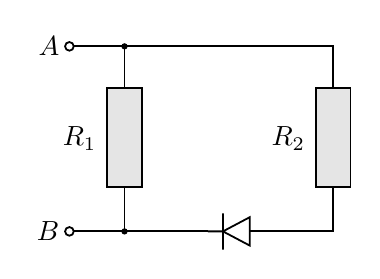
\begin{tikzpicture}[>=stealth,line width=.65pt]\draw (0,2.35)--(3.35,2.35)--(3.35,1.82) (3.35,.56)--(3.35,0)--(2.29,0) (1.76,0)--(0,0) (.7,2.35)--(.7,1.82) (.7,.56)--(.7,0);\draw[fill=gray!20](.48,.56)rectangle(.92,1.82) (3.13,.56)rectangle(3.57,1.82);\draw(2.29,0)--(2.29,.18)--(1.95,0)--(2.29,-.18)--cycle (1.95,.23)--(1.95,-.23) (1.95,0)--(1.76,0);\foreach \p in {(.7,0),(.7,2.35)}{\fill \p circle(.04);}\draw[fill=white](0,0)circle(.055) (0,2.35)circle(.055);\node[left]at(0,2.35){$A$};\node[left]at(0,0){$B$};\node[left]at(.47,1.18){$R_1$};\node[left]at(3.12,1.18){$R_2$};\end{tikzpicture}\end{center}

В цепи, изображённой на рисунке, сопротивление диода в прямом направлении пренебрежимо мало, а в обратном многократно превышает сопротивление резисторов. При подключении к точке A положительного, а к точке B  — отрицательного полюса батареи с ЭДС $6\,\text{В}$ и пренебрежимо малым внутренним сопротивлением потребляемая мощность (тепловая мощность, выделяемая во внешней цепи) равна $13$ Вт. При изменении полярности подключения батареи потребляемая мощность равна $9$ Вт.
Укажите для обоих случаев подключения батареи, протекает ли ток через диод и каждый из резисторов или нет, и определите сопротивления резисторов в этой цепи.
}{
\smallskip\noindent\textbf{Решение}\par
\begin{center}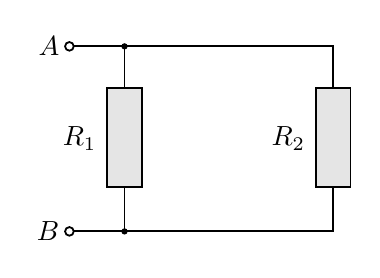
\begin{tikzpicture}[>=stealth,line width=.65pt]\draw (0,2.35)--(3.35,2.35)--(3.35,1.82) (3.35,.56)--(3.35,0)--(0,0) (.7,2.35)--(.7,1.82) (.7,.56)--(.7,0);\draw[fill=gray!20](.48,.56)rectangle(.92,1.82) (3.13,.56)rectangle(3.57,1.82);\foreach \p in {(.7,0),(.7,2.35)}{\fill \p circle(.04);}\draw[fill=white](0,0)circle(.055) (0,2.35)circle(.055);\node[left]at(0,2.35){$A$};\node[left]at(0,0){$B$};\node[left]at(.47,1.18){$R_1$};\node[left]at(3.12,1.18){$R_2$};\end{tikzpicture}\end{center}

 рис. а) 

Если подключить к точке А положительный полюс батареи, а к точке В  — отрицательный, то ток через диод идет. С учетом условия, что в прямом направлении его сопротивление пренебрежимо мало, получаем эквивалентную схему а), в которой два резистора соединены параллельно. Их общее сопротивление находится из формулы 

\[\frac{1}{R} = \frac{1}{R_1} + \frac{1}{R_2} .\]

С учетом, что внутреннее сопротивление батареи пренебрежимо мало, $U= \mathcal{E} ,$ потребляемая мощность равна

\[P_1= \frac{\mathcal{E} ^2}{R} .\]



\begin{center}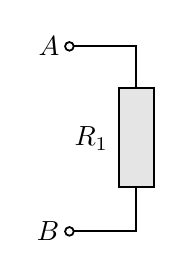
\begin{tikzpicture}[>=stealth,line width=.65pt]\draw (0,2.35)--(.85,2.35)--(.85,1.82) (.85,.56)--(.85,0)--(0,0);\draw[fill=gray!20](.63,.56)rectangle(1.07,1.82);\draw[fill=white](0,0)circle(.055) (0,2.35)circle(.055);\node[left]at(0,2.35){$A$};\node[left]at(0,0){$B$};\node[left]at(.62,1.18){$R_1$};\end{tikzpicture}\end{center}

 рис. б) 

 Если изменить полярность подключения, то ток через диод не пойдет, а, следовательно, не пройдет через резистор $R_{2}$. В этом случае эквивалентная схема будет иметь вид, представленный на рис. б). Мощность тока в этом случае будет равна

\[P_2= \frac{\mathcal{E} ^2}{R_1,}\]

откуда находим сопротивление первого резистора:

\[R_1= \frac{\mathcal{E} ^2}{P_2} = \frac{36}{9} =4\,\text{Ом}.\]

Тогда сопротивление второго резистора равно

\[R_2= \frac{\mathcal{E} ^2}{P_1 - P_2} = \frac{36}{13 - 9} =9\,\text{Ом}.\]

Ответ: $R_1=4\,\text{Ом}; R_2=9\,\text{Ом}.$
}

\end{document}
